\par La méthodologie de la collecte des indicateurs est la suivante: 
\begin{itemize}
    \item La collecte est démarrée après un démarrage frais.
    \item Elle est consolidée dans un seul fichier.
    \item La date et l'heure du début de la collecte sont précisées.
    \item Au moment précis de début et de fin de chacun des tests, une entrée spéciale est ajoutée dans le fichier de collecte des indicateurs avec la date et l'heure, un libellé et une description. Ce point de contrôle (checkpoint) est fait grâce à une commande shell qui vient ajouter une trace dans le fichier de collecte des indicateurs.
    \item Chaque indicateur est collecté aux 5 secondes. Ce délai est réévalué au besoin, selon les fréquences des pics observées. 
\end{itemize}
\par Ensuite tout au long des tests de validations matériels et logiciels les indicateurs sont collectés. 
\par Chaque indicateur est une paire de clé=valeur. Il existe le même nombre d'indicateurs à tout moment. La date et l'heure sont un champ, ainsi que la source (tegrastats, System Monitor, user) et le champ descriptif. 
\par Avant tout début de tests, la collecte est démarrée. Cela permet de prendre une base de référence sans aucune charge.
\par Les indicateurs de performances sont collectés avant les tests matériels et logiciels lors du montage du nano ordinateur. Cela permet d'observer le "payload" possible d'un équipement ou d'un logiciel, sans lien avec l'inférence. Par exemple Chromium. Ou la caméra avec GStreamer. 
\par Ensuite les tests avec l'inférence débutent. D'abord par des tests de régression, pour s'assurer que l'environnement est toujours fonctionnel et retourne les mêmes résultats que les tests similaires précédents, que nos attentes sont respectées. 
\par Puis par des tests ciblés, en commençant par l'inférence avec des images de diverses résolutions. Et pour finir par l'inférence avec des vidéos de diverses résolutions. 
\par Les indicateurs collectés permettent de créer des graphiques qui montrent la progression de chacun avant, pendant et après le test.  Le min, max et avg peut être extrait.
\par Les performances matérielles du Jetson Nano sont évaluées grâce au System Monitor d’Ubuntu et les métriques tegrastats fournis par NVidia.
\par Les performances de la segmentation sont évaluées grâce au IoU et au z-score pour la classe du chemin / route. Une fonction Python est utilisée. Les fonctions IoU et le z-score utilisent l'image prédite (généré par le modèle FCN) et l'image Ground Truth. Les images originales sont donc présélectionnées selon leur intérêt et l'image Ground Truth créée. L'image prédite et Ground Truth doivent utiliser la même palette de couleurs et doivent être de la même résolution. 
L'image Ground Truth est créée à la main avec l'éditeur Gimp. Comme la segmentation de l'image prédite par le modèle de NVidia est très carrée, l'image Ground Truth ne sera pas précise au pixel prêt. Le besoin est d'évaluer et non d'entrainer, l'importance de la précision de la classification est moindre. 

\label{metho_eval}
\begin{figure}
    \centering
    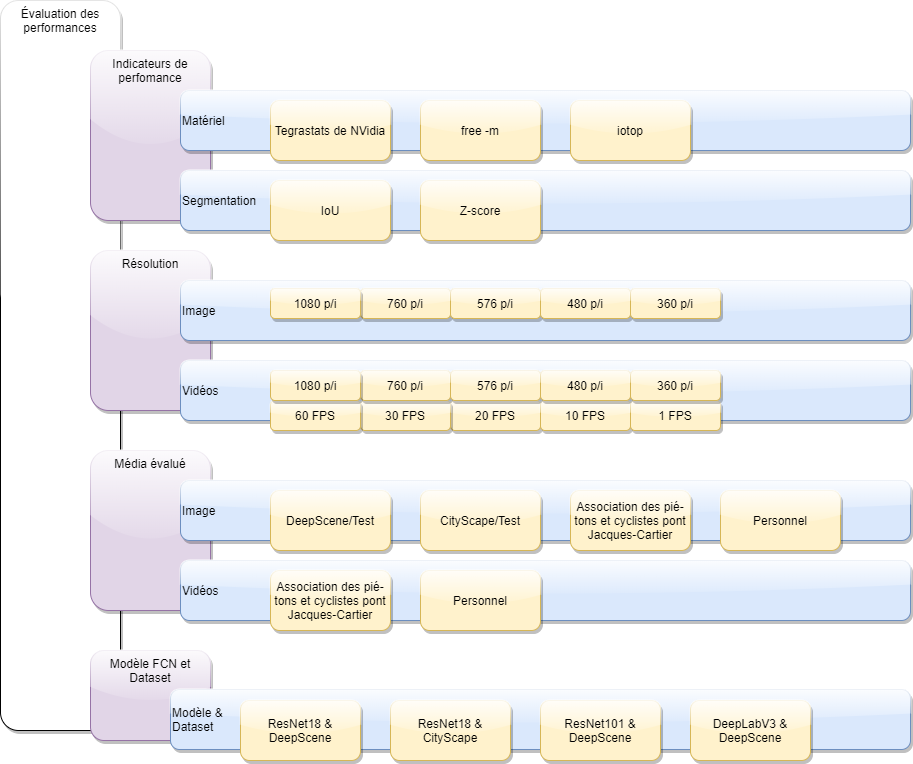
\includegraphics[width=1.0\textwidth]{metho_eval_perf_round_glass_shadow.png}
    \caption{Méthodologie de l'évaluation des performances}
    \label{fig:metho_eval}
\end{figure}
